\documentclass{article}
\usepackage[utf8]{inputenc}
\usepackage{graphicx}
\usepackage{enumerate}
\usepackage{amsmath}

\graphicspath{ {images/} }

\setlength{\parskip}{1em}
\renewcommand{\baselinestretch}{1.3}

\renewcommand{\theenumi}{\roman{enumi}}
\usepackage{enumerate}
\graphicspath{ {../figs/} }

\setlength{\parskip}{1em}
\renewcommand{\baselinestretch}{1.3}

\begin{titlepage}
    \begin{center}
        \Huge
        \textbf{Programming Finite Element Method}
        \vspace{0.5cm}

        \Large
        Earth 409: Earth System Modeling Course Project\\
        \vspace{0.5cm}
         
        \normalsize
        By: \textbf{Prithvi Thakur}\\
        Date: December 14th, 2018
    \end{center}
\end{titlepage}

\begin{document}

\section{Introduction}
Most partial differential equations with more than one variable usually can not be solved analytically. We learnt finite difference methods in the course where we approximate the derivatives of the solution as a Taylor series expansion of space and time discretizations. This method transforms the partial differential equation into a system of algebraic equations which can be solved easily. 

While the finite difference methods are easier to implement, they do not work well for the cases with complex geometry. Some examples would include systems with complicated boundary conditions which can not be represented analytically, but can be represented as a piece-wise continuous function. Another example where finite element methods would outperform finite differences is when we have variable material properties (rigidity, bulk modulus, density, etc) in space.

\begin{figure}[!htb]
    \centering
    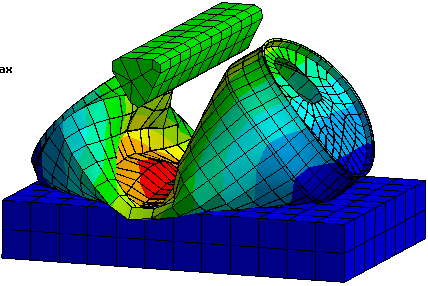
\includegraphics[scale=0.5]{fig1.png}
    \caption{Stress contours of a deformed can[1]. Such a complex geometry is difficult to implement in finite difference or pseudospctral methods.}
\end{figure}

In this project, I explain the concept and implementation behind the finite element methods in one dimension. We will work with a simple one dimensional Navier-Stokes equation, which is useful in the applications of linear elasticity, e.g., stresses on a rod.

\section{Linear Elasticity: Navier-Stokes in one dimension}
Consider a rod of finite length made of linearly elastic material. We consider the rod to be in steady state, i.e., a load was applied slowly enough so that there is no acceleration anywhere on the rod, and it was applied sufficiently long ago so that all the vibrations have died out. The fundamental equations for static response of the elastic rod are [2]:
\begin{itemize}
    \item The divergence of stress ($\sigma$) is balanced by the body forces($b$): equilibrium equation
    \item The stress ($\sigma$) is related to the strain($\varepsilon$) in a linear manner: material constitutive equation
    \item The strain($\varepsilon$) is given by the displacement($u$) gradient: strain definition
\end{itemize}

These equations can be written as:

\begin{align}
    \centering
    \frac{d\sigma}{dx} + b &= 0 \\
    \sigma &= \varepsilon E \\
    \varepsilon &= \frac{du}{dx} 
\end{align}

We substitude stress and strain in the equilibrium equation to get an expression relating displacement to elastic properties. We get:
\begin{align}
    \frac{d^2u}{dx^2} + \frac{b}{E} = 0
\end{align}

For simplicity, we consider the forcing term to be one, therefore the equation becomes 
\begin{align}
    -\frac{d^2u}{dx^2} = 1
\end{align}

Since this equation is second order in $x$, we need two boundary conditions to compute the solution. I will use a fixed (zero) displacement boundary on the two sides of the finite rod. Let the rod be a unit length placed in a cartesian coordinate system with its left end placed at $x = 0$ and parallel to the $x$ axis. We can write the differential equation with its boundary conditions and the domain as:
\begin{align}
    -\frac{d^2u}{dx^2} = 1;\ x_{\epsilon}[0,1];\ u(0) = u(1) = 0 \\
    -u^{''}(x) = 1; \ x_{\epsilon}[0,1];\ u(0) = u(1) = 0 
\end{align}


\section{Methodology}
The idea behind finite element methods is to break up the domain into multiple elements, and calculate the solution for each element at a local level. In order to do this efficiently, we can represent our solution $u(x)$ as a set of piecewise functions with the property that these functions are zero outside the element in consideration. These are known as basis functions. Using this expansion and some variational calculus, we can transform our equation into a set of ordinary differential equations which can be solved using linear algebra.

As with all other numerical methods, we start with a mesh discretization of the space. We use linearly spaced elements inside the domain $[-1,1]$. Let the number of elements be $M$. 

Next, we need to define the basis functions. For simplicity, we use a simple hat function as our basis function. More complicated higher order basis functions can be used if the geometry is curved or non-planar. Fig. 2. shows a typical example of the hat basis function[2]. One of the biggest advantages of finite element method is that the basis functions are piecewise, therefore elements with non-uniform size will be just as easy to work with as elements with uniform size. This is because we are essentially solving for each element within the domain of the basis functions, e.g. [0,1] for hat functions. 

\begin{figure}[!htb]
    \centering
    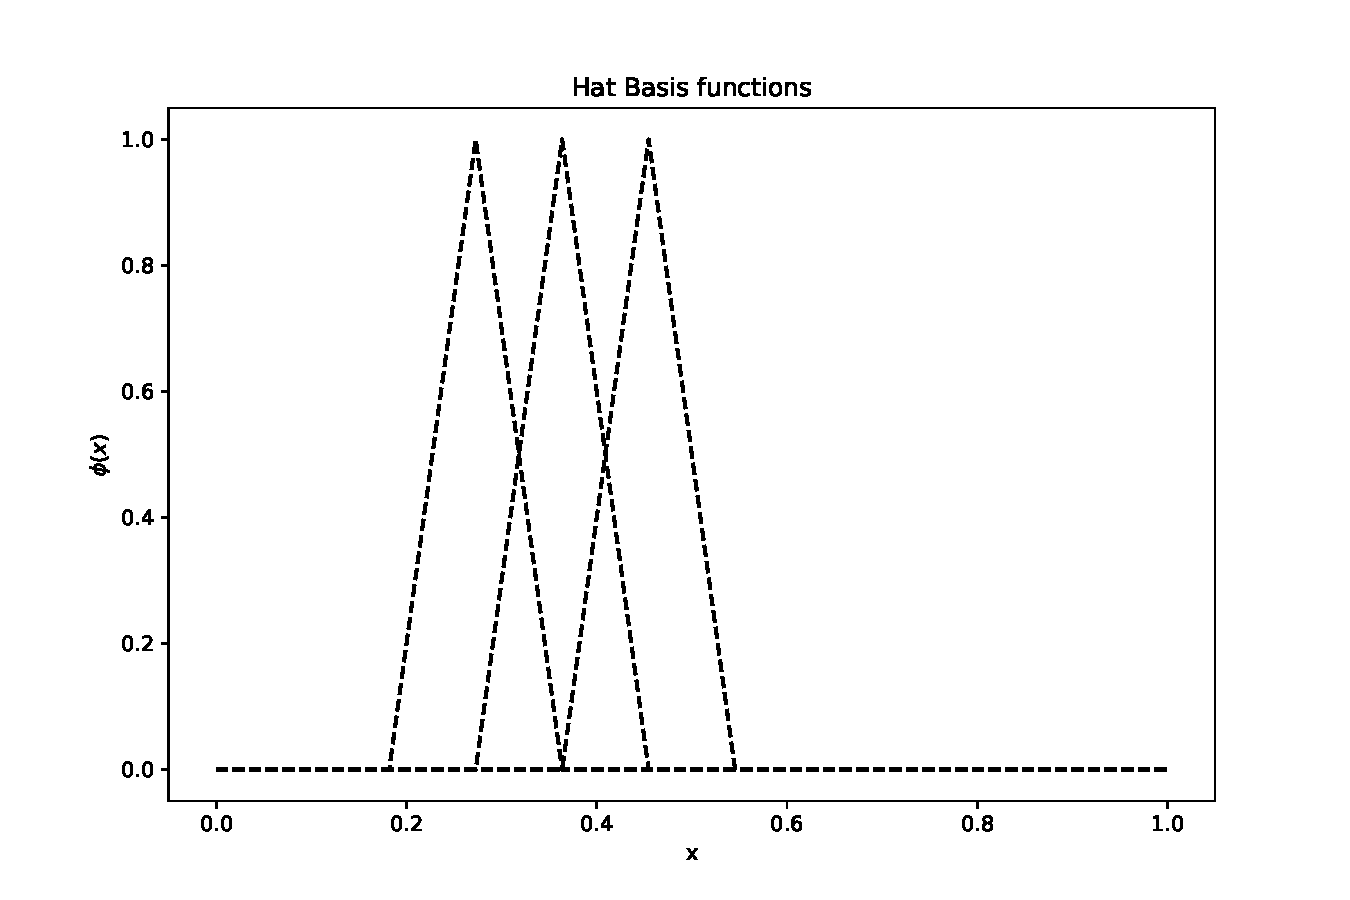
\includegraphics[scale=0.5]{fe_basis1.pdf}
    \caption{Hat basis functions for three consecutive elements. The values are non zero only for the element in consideration, and zero everywhere else. In this example, we consider simplest basis function. But we may have the elements further discretized into several nodes and the basis function can be higher order polynomials interpolated over the nodes.}
\end{figure}

The next step is to derive the weak or the variational form of the differential equation. This is a two-step process: first, we multiply our differential equation with a test function, and second, we integrate the equation by parts to get rid of the derivatives of the solution. There are multiple choices for the test function, and different choices lead us to very different methods using the same formulation. If our test function is a dirac delta function, we end up with pseudospectral methods for solving partial differential equations. For finite element methods, we will let the test function be same as the basis functions we chose to approxiamte the solution. This is called the Galerkin method, and is proven to be much better than other choices [3]. The most obvious advantage of using test function the same as the basis function is that they are orthogonal, therefore unless the element is same, the product of two such functions is zero. This results in sparse matrices for inverting the solutions.

Multiplying our solution with a test function $v$, integrating by parts within the domain,and applying Green's theorem gives us:
\begin{align}
    -u^{''}v = fv;\ &where\ f = 1. \\
    -\int_{0}^{1}u^{''}vdx &= \int_{0}^{1}fvdx \\
    -\int_{0}^{1}u^{'}vdx + \int_{0}^{1}u^{'}v^{'} dx &= \int_{0}^{1}fvdx \\
    \int_{0}^{1}u^{'}v^{'} dx &= \int_{0}^{1}fvdx 
\end{align}

The reason for using this formulation is mostly historic and a matter of convention. Finite element methods were developed by structual engineers and fluid dynamicists and the conservation of certain physical field quantities are easily represented by the variational formulation.

For a set of basis functions $\phi(x)$, our solution $u(x)$ can be written as $u(x) = \sum_{j=1}^{M}c_j\phi_j(x)$. Here $c_j$ are the unknown coefficients to be determined. Substituting this in equation 11, we get
\begin{align}
    \int_{0}^{1}\sum_{j=1}^{M}c_j\phi_j^{'}(x)v^{'} dx =
    \sum_{j=1}^{M}\int_{0}^{1}c_j\phi_j^{'}(x)v^{'} dx =
    \int_{0}^{1}fvdx 
\end{align}

Next, we choose the test function $v(x) = \phi_1, \hdots, \phi_M-1$ successively so as to get $M-2$ independent equations. These equations, together with the boundary conditions will be sufficient to determine the coefficients $c_j$ for the solution.
\begin{align}
    \left( \int_0^1 \phi_1^{'}\phi_1^{'}dx\right)c_1 + \hdots + \left( \int_0^1 \phi_1^{'}\phi_{M-1}^{'}dx \right)c_1 &= \int_0^1 f\phi_1dx     \\
    \left( \int_0^1 \phi_2^{'}\phi_1^{'}dx\right)c_1 + \hdots + \left( \int_0^1 \phi_2^{'}\phi_{M-1}^{'}dx \right)c_1 &= \int_0^1 f\phi_2dx     \\
    \vdots  \\
    \left( \int_0^1 \phi_{N-1}^{'}\phi_1^{'}dx\right)c_1 + \hdots + \left( \int_0^1 \phi_{N-1}^{'}\phi_{M-1}^{'}dx \right)c_1 &= \int_0^1 f\phi_{N-1}dx
\end{align}

We can write the above set of equations in matrix form as follows:
\begin{align}
    \begin{bmatrix}
        a(\phi_1,\phi_1) & a(\phi_1,\phi_2) & \hdots \\
        \vdots      &   \ddots      &       \vdots \\
        a(\phi_{M-1},\phi1) & \hdots    & a(\phi_{M-1},\phi_{M-1})
    \end{bmatrix}
    \begin{bmatrix}
        c_1 \\
        \vdots \\
        c_{M-1}
    \end{bmatrix}
    =
    \begin{bmatrix}
        <f,\phi_1> \\
        \vdots \\
        <f,\phi_{M-1}>
    \end{bmatrix}
\end{align}

where,
\begin{align}
    a(\phi_i,\phi_j) = \int_0^1 \phi_i^{'}\phi_j^{'}dx, \\
    <f,\phi_i> = \int_0^1 f\phi_i dx
\end{align}

If the basis functions arehat functions, we get:
\begin{align}
    \begin{bmatrix}
        \frac{2}{h} & \frac{-1}{h} & \hdots \\
        \frac{-1}{h} & \frac{2}{h} & \frac{-1}{h} \\
        \hdots & \frac{-1}{h} & \frac{2}{h}
    \end{bmatrix}
    \begin{bmatrix}
        c_1 \\
        \vdots \\
        c_n
    \end{bmatrix}
    =
    \begin{bmatrix}
        \int_0^1 f\phi_1 dx \\
        \vdots \\
        \int_0^1 f\phi_{M-1} dx
    \end{bmatrix}
\end{align}

Thus, assembling the left hand matrix is straightforward. To compute the right hand side of the matrix, we need tointegrate the given function over the basis function. We can use any integration algorithm like quadrature integration or simpson's rule. I have imported simpson's method from python'sscipy library to compute the right hand side.

\section{Results}
I have implemented the above method in python. The right hand side of equation (20) is computed using simpson's rule for integration. The function $f$ in our case is 1. The basis functions can be programmed using the following formulation for the $i^{th}$ basis function:
\begin{align}
    \phi_i(x) = \left\{
        \begin{matrix}
            0 & x < x_{i-1} \\
            \frac{x-x_{i-1}}{\Delta x} & x_{i-1} \le x < x_i \\
            1 - \frac{x - x_i}{\Delta x} & x_i \le x < x_{i+1} \\
            0 & x > x_{i+1}
        \end{matrix}
\end{align}

We solve the system of linear equation using numpy's linear solver {\tt numpy.linalg.solve()}. We compare the finite element solution of a one-dimensional Navier-Stokes equation with it's analytically computed solution in Fig. 3. The errors are shown in Fig. 4.

\begin{figure}[!htb]
    \centering
    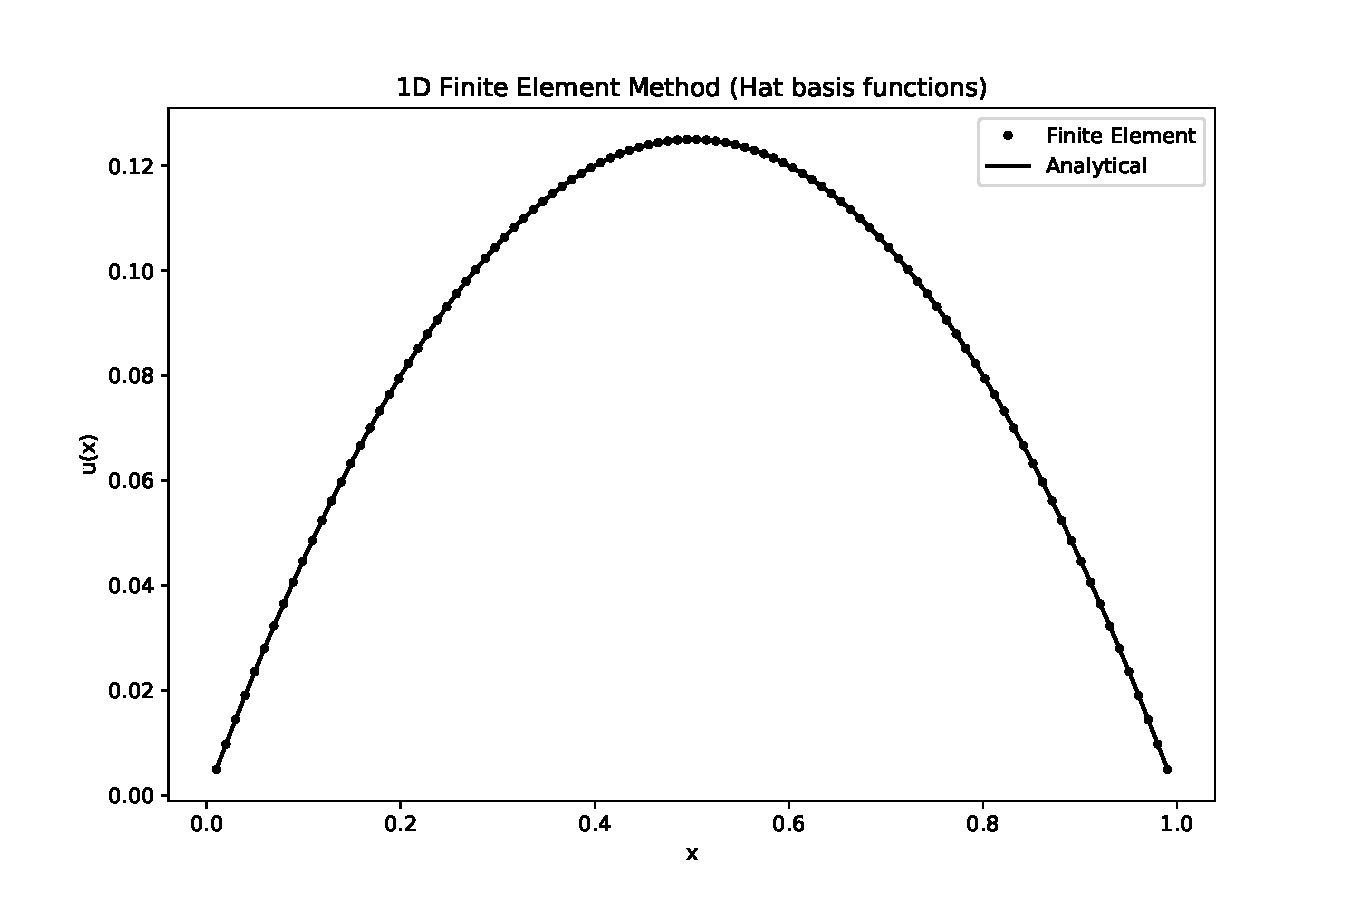
\includegraphics[scale=0.45]{fe_sol.pdf}
    \caption{Analytically computed solution vs. the finite element solution. We can see that there is a pretty good match even at the boundaries.}
\end{figure}
\begin{figure}[!htb]
    \centering
    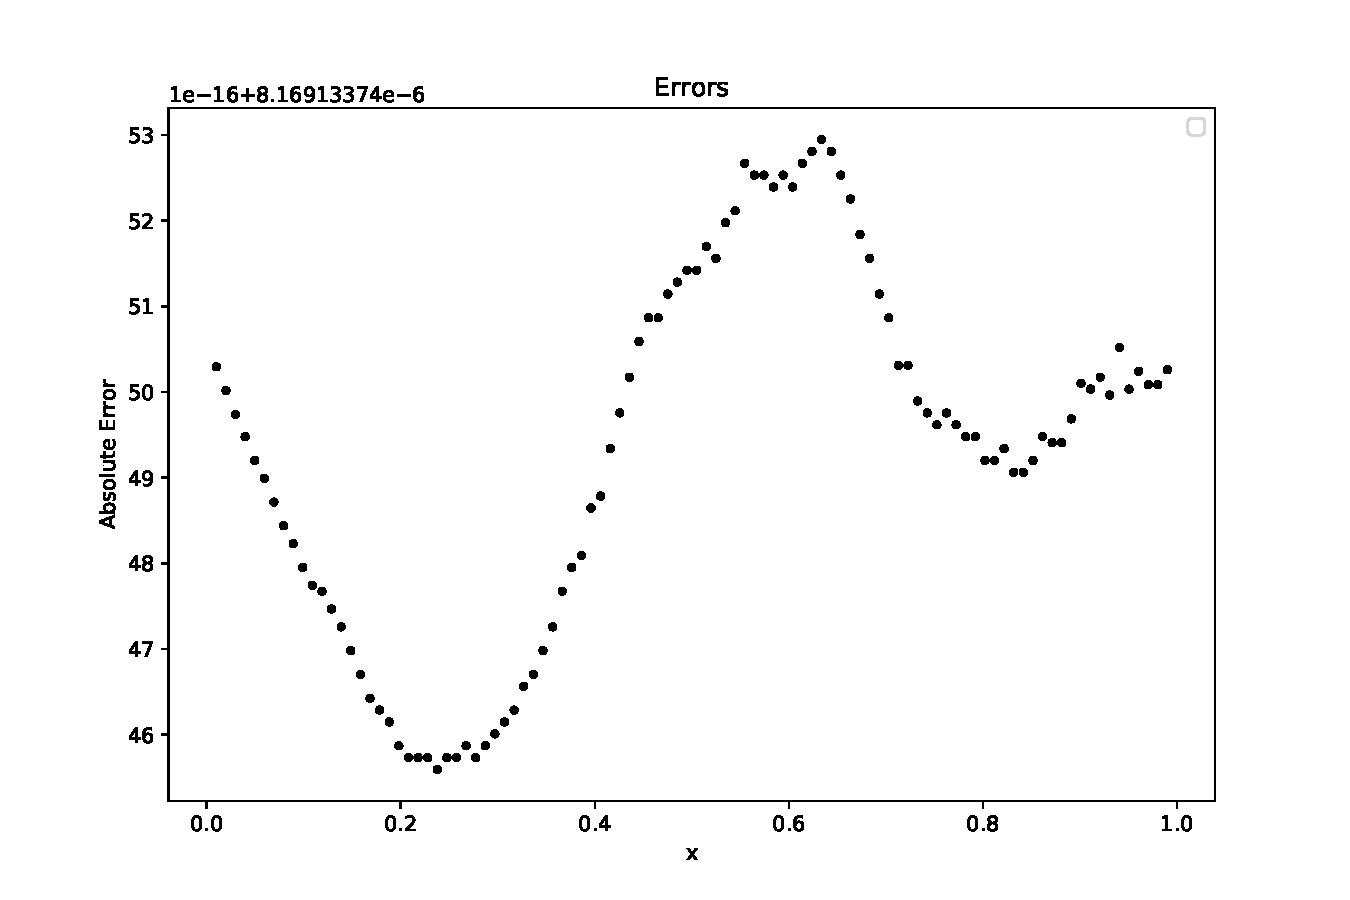
\includegraphics[scale=0.45]{fe_err.pdf}
    \caption{The errors in the finite element solution. These are in the order of $10^{-6}$, which is greater than the machine precision error. The errors would be significantly reduced if we used higher order basis functions.}
\end{figure}

\section{References}
$[1]$ http://faculty.washington.edu/nsniadec/ME478/S13/ \\* 
$[2]$ Achenbach, J. (2012). Wave propagation in elastic solids (Vol. 16). Elsevier.\\*
$[3]$ https://www.wikiwand.com/en/Galerkin\_method. \\*

\end{document}
